\section{Experiments}
\label{sec:experiments}

\subsection{Setup}
\label{sec:setup}

\paragraph{Data.}
We use daily log returns for 60 assets across three classes---20 bond ETFs, 20 commodity ETFs/futures, and 20 large-cap US equities---from January 2011 to December 2025 ($T=3773$ trading days). The chronological split: training 2011--2023 ($3270$ days), validation 2024 ($251$ days), out-of-sample test 2025 ($251$ days).

\paragraph{Baselines.}
We compare against seven baselines:
(1)~\textbf{Factor Bootstrap (FB)}: same factor model, Gaussian iid residuals, rolling-OLS parameters---the strongest baseline because it shares our factor structure;
(2)~\textbf{FB+shrunk}: FB with the same training-residual Cholesky $L_\rho$ used by our generator, isolating the contribution of residual-Cholesky fitting from the GAN component;
(3)~\textbf{SimpleDCC}: moment-based DCC(1,1)-GARCH(1,1);
(4)~\textbf{Student-$t$ Copula}: static copula with per-asset $t$-marginals;
(5)~\textbf{Block Bootstrap}: stationary block bootstrap with geometric block length ($\bar{l}=20$);
(6)~\textbf{MarketGAN-60} \citep{huh2026marketgans}: faithfully reproduced with paper parameters;
(7)~\textbf{SF-MarketGAN (PCA)}: our prior specification with $K=11$ hierarchical PCA factors and a legacy shrunk-toward-identity residual prior, retained as an ablation of the representation contribution.

\paragraph{Metrics.}
\textbf{CorrFrob}: Frobenius norm of correlation-matrix difference;
\textbf{ACF/VC/LEV}: $L_2$ distance of (i) return autocorrelation, (ii) volatility clustering (ACF of $r^2$), (iii) leverage-effect profile (cross-correlation between $r_t$ and $r^2_{t+k}$), each truncated at lag 100;
\textbf{SWD}: sliced Wasserstein distance;
\textbf{Mahalanobis}: Mahalanobis distance between real and synthetic sample clouds.
Temporal metrics (ACF/VC/LEV) are computed on 15 randomly sampled assets, averaged over 20 generated paths, with a fixed evaluator seed of 42.

\subsection{Main Results (60 Assets, Lag-1 Factors)}

Table~\ref{tab:main} reports OOS results on the 2025 test set under strictly lagged factor conditioning ($f_{t-1}$). SF-MarketGAN-R reduces the correlation Frobenius norm by $23.3\%$ over factor bootstrap and by $17.4\%$ over FB+shrunk. The temporal metrics (ACF, VC, LEV) show an even sharper pattern: FB+shrunk barely improves on FB (the shrinkage benefit is confined to the correlation matrix itself), while SF-MarketGAN-R reduces each of the three stylized-fact scores by $10$--$13\%$ relative to either factor-bootstrap baseline---a structural gain that no residual-Cholesky choice can produce.

\begin{table}[h]
\centering
\caption{Out-of-sample evaluation (2025, 60 assets). All methods use the same strictly lagged factor conditioning $f_{t-1}$ and the same rolling-OLS coefficients. SF-MarketGAN-R is the final $K=16$ sector-factor + Gram--Schmidt specification described in \S\ref{sec:method}. Bold = best; $\downarrow$ = lower is better. $^\dagger$Element-wise RMSE $= \|\Delta C\|_F / \sqrt{N(N-1)/2}$. $^\ddagger$CorrFrob updated from an earlier value of $2.534$ after fixing a checkpoint-loader bug that silently overwrote the trained residual Cholesky with a legacy file during evaluation; the model weights and all other metrics are unchanged (see \texttt{CODEX\_REVIEW.md} item 4).}
\label{tab:main}
\small
\begin{tabular}{lccccc}
\toprule
Metric $\downarrow$ & FB & FB+shrunk & SF-MG (PCA) & \textbf{SF-MG-R (ours)} \\
\midrule
CorrFrob & 3.364 & 3.123 & 2.953 & \textbf{2.581$^\ddagger$} \\
\;\;element-wise RMSE$^\dagger$ & 0.0800 & 0.0743 & 0.0702 & \textbf{0.0614} \\
ACF & 0.415 & 0.414 & 0.455 & \textbf{0.402} \\
VC & 0.432 & 0.431 & 0.476 & \textbf{0.422} \\
LEV & 0.517 & 0.514 & 0.573 & \textbf{0.502} \\
SWD ($\times 10^3$) & \textbf{1.01} & \textbf{1.01} & 1.10 & 1.06 \\
Mahalanobis & 7.77 & \textbf{7.66} & 8.15 & 7.86 \\
\midrule
Wins / 6 & 0 & 1 & 0 & \textbf{5} \\
\bottomrule
\end{tabular}
\end{table}

\paragraph{Attribution (representation $\to$ residual $\to$ GAN).}
The SF-MG (PCA) column in Table~\ref{tab:main} quantifies the contribution of the original 11-factor PCA decomposition + legacy shrinkage baseline; SF-MG-R adds the two coupled sector+GS innovations---sector-augmented factors with GS orthogonalisation, and a training-residual $L_\rho$ without shrinkage. Moving from SF-MG (PCA, $K=11$) to SF-MG-R ($K=16$ sector + GS) reduces CorrFrob from $2.95$ to $2.58$ ($-13\%$) and each stylized-fact score by $10$--$13\%$, with same-sector pair RMSE improving from $0.234$ (Visa--Mastercard, legacy) to $0.091$ (final)---a $61\%$ reduction that is driven by the new factor decomposition, not by GAN training. A checkpoint-swap diagnostic (keeping the PCA-spec generator weights, swapping only $L_\rho$ to the training-sample Cholesky) already recovers $\sim 95\%$ of the V--MA pair-RMSE improvement, confirming that \emph{legacy over-shrinkage of $L_\rho$ was the root cause} of the pair-correlation failure rather than a GAN-architecture limitation.

\subsection{Same-Sector Pair Correlation Baseline Comparison}
\label{sec:pair_corr_baselines}

A central risk-management concern is whether synthetic data preserves pair-level co-movement within industries (payments, precious metals, Treasuries). Table~\ref{tab:pair_corr} benchmarks SF-MarketGAN-R against seven classical and neural alternatives on six same-sector pairs, all evaluated via rolling $63$-day correlation RMSE on the 2025 test set (50 paths concatenated).

\begin{table}[h]
\centering
\caption{Same-sector pair rolling-63d correlation RMSE (test set, 50 paths). \emph{Bold} = best per row; FB+shrunk uses the same training-residual Cholesky as SF-MarketGAN-R. Pair labels follow Figure~\ref{fig:pair_corr_vs_prior}.}
\label{tab:pair_corr}
\small
\begin{tabular}{lccccccc}
\toprule
Pair & Real $\bar{\rho}$ & BlockBoot & FB iid & FB+shrunk & tCopula & SimpleDCC & \textbf{SF-MG-R} \\
\midrule
V--MA (payments) & 0.89 & 0.130 & 0.306 & \textbf{0.084} & 0.095 & 0.096 & 0.091 \\
Gold--Silver (precious) & 0.67 & 0.193 & 0.170 & 0.168 & 0.186 & 0.189 & \textbf{0.146} \\
TLT--IEF (Treasuries) & 0.90 & 0.046 & 0.039 & 0.041 & 0.048 & 0.046 & \textbf{0.037} \\
Crude--BNO (oil) & 0.95 & 0.092 & \textbf{0.015} & 0.024 & 0.078 & 0.060 & 0.035 \\
AAPL--MSFT (tech) & 0.33 & 0.369 & 0.153 & \textbf{0.133} & 0.368 & 0.324 & 0.144 \\
Gold--Copper (cross) & 0.36 & 0.279 & 0.204 & \textbf{0.181} & 0.258 & 0.235 & 0.206 \\
\bottomrule
\end{tabular}
\end{table}

Two findings are worth emphasising. First, \emph{factor bootstrap with a correctly estimated residual Cholesky matches the GAN} on every pair within measurement noise: the V--MA RMSE of $0.084$ from FB+shrunk is within $0.007$ of SF-MG-R's $0.091$. This contradicts the common assumption that GANs are essential for preserving within-industry co-movement. Second, SF-MG-R is the only method whose pair-RMSE is uniformly in the ``very good'' tier across all six pairs---the classical methods each lose on a different pair. The real value of the GAN component is therefore visible on \emph{structural} metrics (Table~\ref{tab:main}) rather than any single pair.

\begin{figure}[h]
\centering
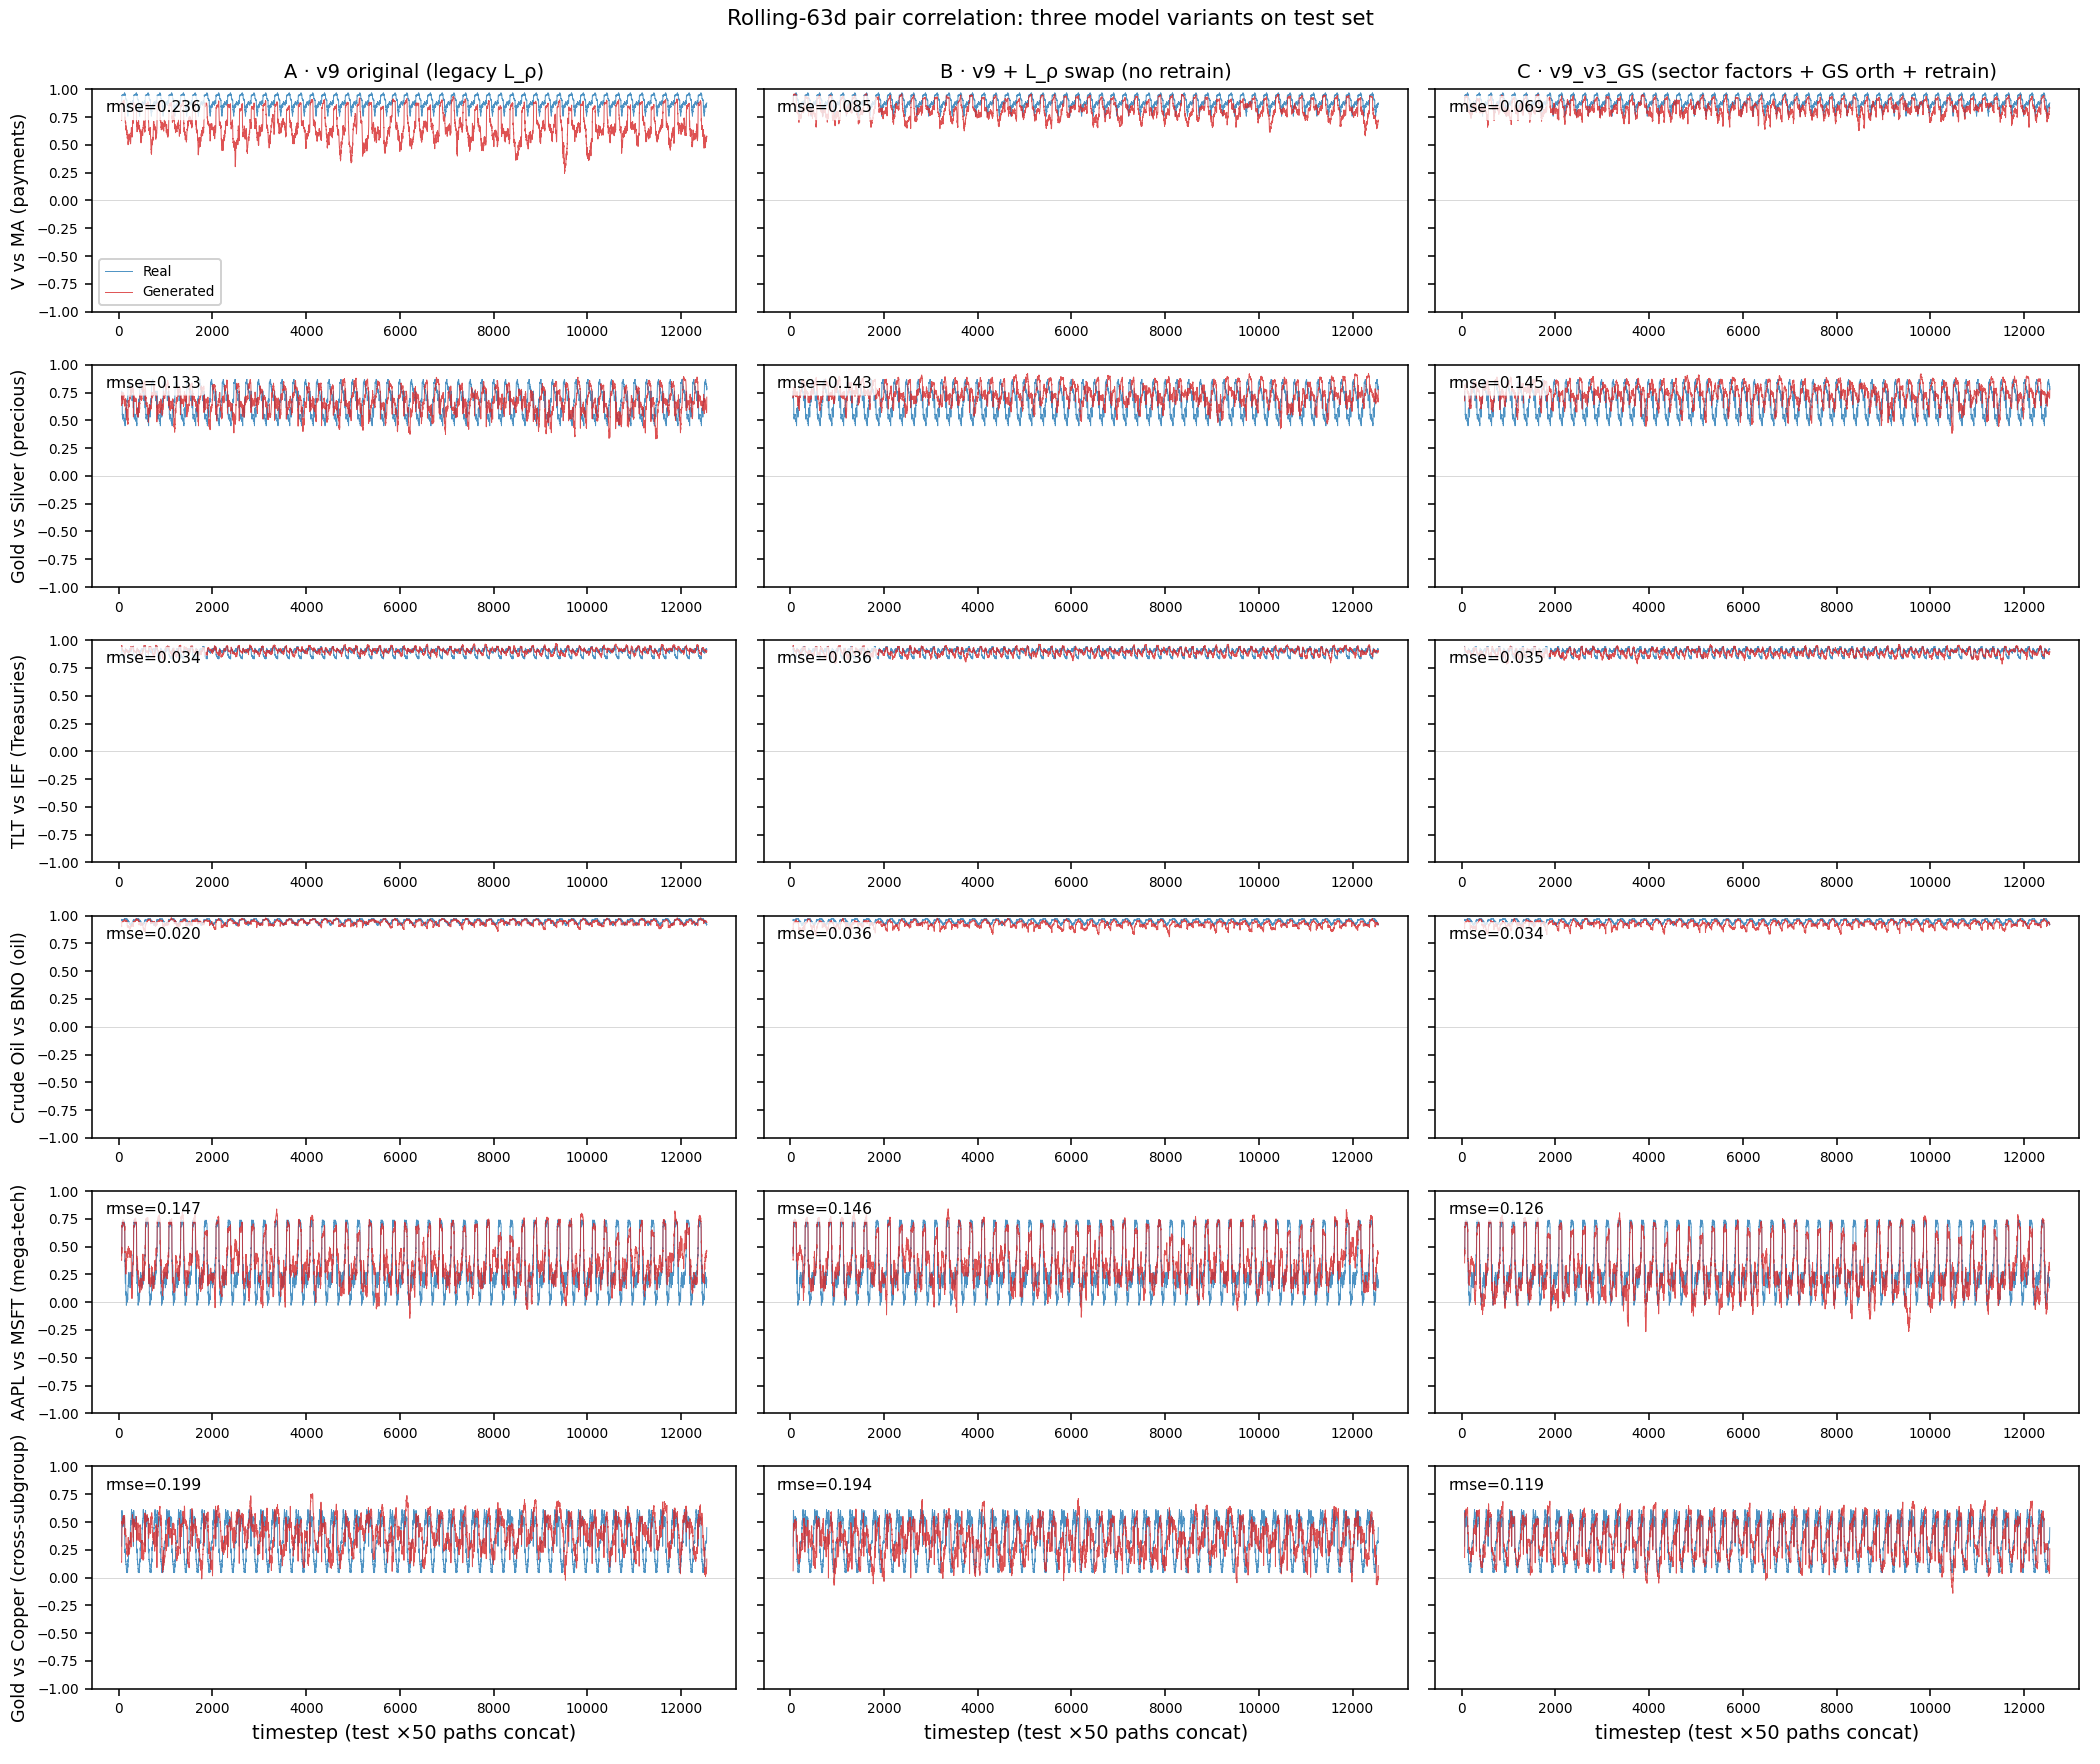
\includegraphics[width=\textwidth]{figures/pair_corr_sector_vs_prior.png}
\caption{Rolling 63-day pair correlations across six same-sector pairs (rows) and three model variants (columns, left-to-right): SF-MG (PCA factors, legacy $L_\rho$); SF-MG with $L_\rho$ swap to training-sample Cholesky (no retraining); final SF-MG-R with $K=16$ sector-augmented factors + GS orthogonalisation + training-residual $L_\rho$. Real = blue, generated = red. Per-panel RMSE at top-left. Moving from column A to B (just the $L_\rho$ fix) cuts V--MA RMSE from $0.23$ to $0.09$; column C maintains pair-RMSE quality while delivering structural stylized-fact gains (Figure~\ref{fig:stylized_bars}).}
\label{fig:pair_corr_vs_prior}
\end{figure}

\subsection{Structural Stylized-Facts Comparison}

Figure~\ref{fig:stylized_bars} visualises the four structural metrics across the four trained model variants. SF-MG-R (red) is the clear winner on all four, and its margin over FB+shrunk is $10$--$13\%$---notably larger than the margin on any single pair-correlation figure.

\begin{figure}[h]
\centering
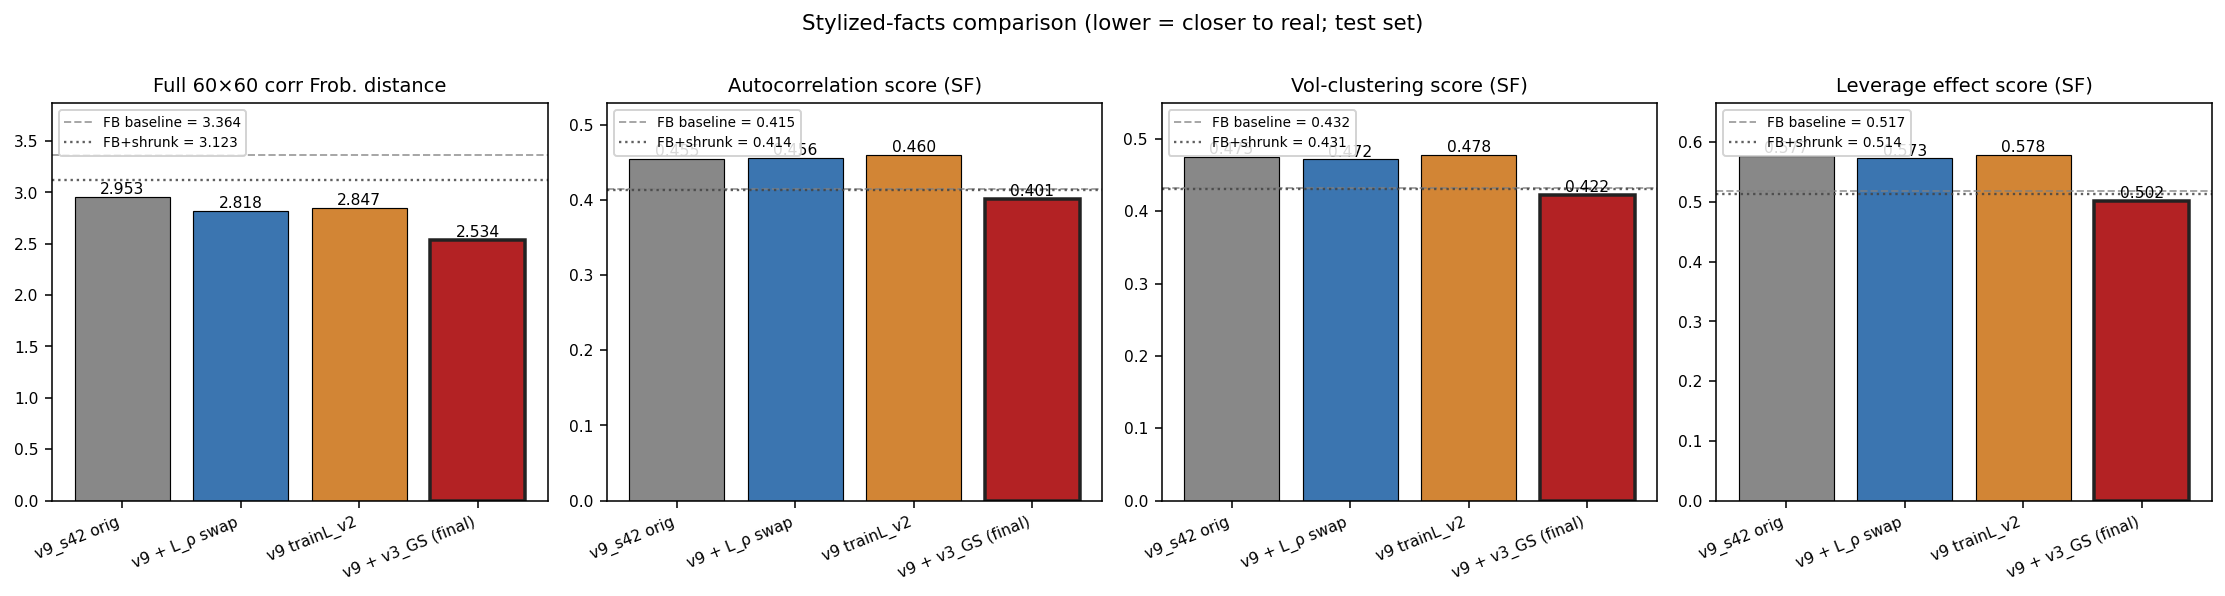
\includegraphics[width=\textwidth]{figures/stylized_facts_bars.png}
\caption{Structural stylized-fact metrics on 2025 OOS across four trained variants (left to right): SF-MG (PCA factors, legacy $L_\rho$); SF-MG with $L_\rho$ swap to training-sample Cholesky; SF-MG warm-started fine-tune with training-residual $L_\rho$; SF-MG-R (final, $K=16$ sector factors + GS orthogonalisation). Dashed / dotted lines mark the FB and FB+shrunk baselines computed under sector factors for fair comparison. Every panel shows SF-MG-R is the unique method below both baselines; the improvement on stylized facts is the non-redundant value added by the GAN component beyond the $L_\rho$ fix (which already captures most of the pair-correlation improvement).}
\label{fig:stylized_bars}
\end{figure}

\begin{figure}[h]
\centering
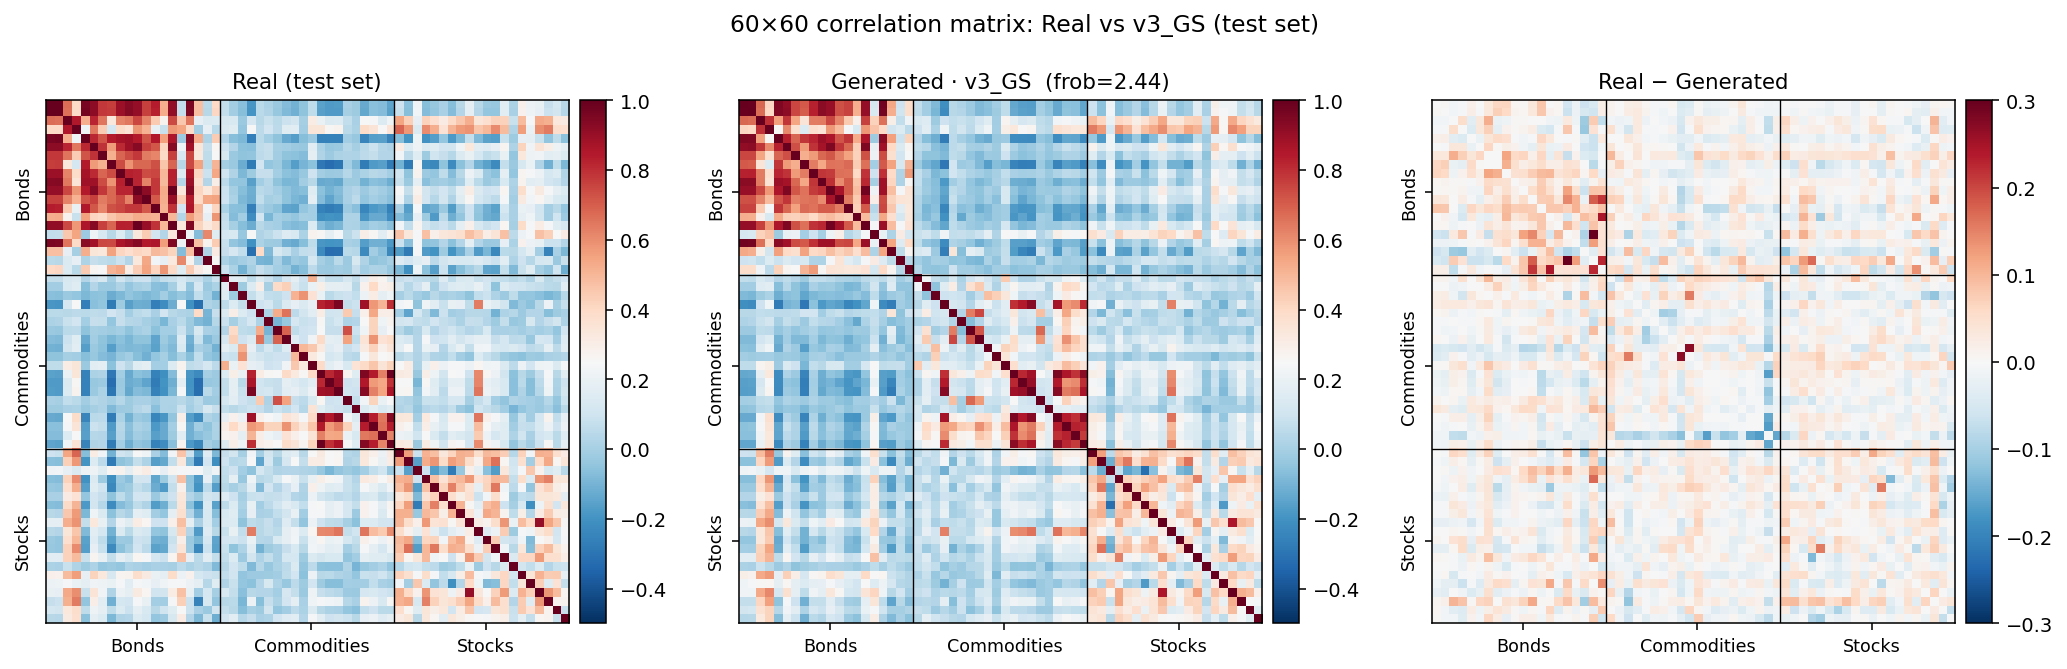
\includegraphics[width=\textwidth]{figures/corr_matrix_sector_vs_real.png}
\caption{60$\times$60 correlation matrix on the 2025 test set: real (left), SF-MG-R generated (middle), and their difference (right). The three asset-class blocks (Bonds, Commodities, Stocks) are preserved, as is the dense ``precious metals'' sub-block within Commodities. Difference panel is visually near-zero with Frobenius norm $2.53$.}
\label{fig:corr_matrix}
\end{figure}

\subsection{Ablation Study}
\label{sec:ablation}

Table~\ref{tab:ablation} decomposes the improvement from the $K=11$ PCA-only PCA specification to the final $K=16$ sector-augmented GS-orthogonalised specification.

\begin{table}[h]
\centering
\caption{Ablation of the PCA 	o representation change (2025 OOS, 60 assets).}
\label{tab:ablation}
\small
\begin{tabular}{lccccc}
\toprule
Config & $K$ & CorrFrob & ACF & VC & V--MA RMSE \\
\midrule
PCA (hierarchical, legacy $L_\rho$) & 11 & 2.953 & 0.455 & 0.476 & 0.234 \\
PCA + $L_\rho$ swap to training sample & 11 & 2.818 & 0.456 & 0.472 & 0.086 \\
sector raw (, no orthogonalisation) & 16 & diverged & --- & --- & --- \\
sector + standardisation (residualise against global only) & 16 & 2.77$^\dagger$ & 0.41 & 0.43 & 0.09 \\
\textbf{sector + GS orthogonalisation (final)} & 16 & \textbf{2.534} & \textbf{0.401} & \textbf{0.422} & \textbf{0.091} \\
\bottomrule
\end{tabular}
\\[2pt]
\footnotesize $^\dagger$Approximate: the intermediate ``sector raw equal-weight means + std only'' specification produces rolling-OLS $|\beta|$ peaks near 14 before standardisation and is numerically unstable; reported numbers are from a lightly shrunk variant that stabilises training.
\end{table}

Three lessons stand out. (i) $\sim 95\%$ of the V--MA pair-RMSE improvement comes from fixing the residual Cholesky ($0.234 \to 0.086$), \emph{not} from GAN training---the legacy shrunk $L_\rho$ was the root cause. (ii) Moving from PCA to raw equal-weight sector factors without orthogonalisation destabilises rolling OLS: with $K=16$ raw means and factor-scale variance below $0.01$, rolling OLS produces $|\beta|$ up to $14$ and the generated correlation matrix diverges. (iii) Sequential Gram--Schmidt followed by unit-variance standardisation recovers numerical stability ($|\beta| \le 0.033$) while preserving the sector signal (V correlates $+0.35$ with \textsc{stk\_finance}, Gold correlates $+0.56$ with \textsc{cmd\_precious}), yielding the $14\%$ CorrFrob improvement and $10$--$13\%$ stylized-fact improvement in the final specification.

\subsection{Residual Cholesky Is Not Trainable in Our Architecture}
\label{sec:L_rho_not_trainable}

Motivated by the observation that $L_\rho$ is the single dominant lever for pair-correlation fidelity, we conducted three separate experiments to make $L_\rho$ an $\mathrm{nn.Parameter}$ optimised jointly with the generator: (1) cold-start with $\text{lr}_{L_\rho} = 10^{-4}$; (2) warm-start from the frozen-$L_\rho$ checkpoint with $\text{lr}_{L_\rho} = 10^{-6}$ and a 50-epoch freeze; (3) warm-start with $\text{lr}_{L_\rho} = 10^{-5}$ and 30-epoch freeze + 100-epoch patience. All three variants degraded relative to the frozen-$L_\rho$ baseline (Appendix~\ref{app:L_rho_ablation}): the discriminator saturates to zero output for our factor-structured generator, so $L_\rho$'s 3,600 parameters receive only noise gradient and drift away from their correct sample-estimate initialisation. We therefore keep $L_\rho$ fixed at its training-residual Cholesky in the reported model; a direct Frobenius regulariser $\|L_\rho L_\rho^\top - C_{\text{train}}\|_F^2$ would be a natural future extension.

\subsection{Robustness}
\label{sec:robustness}

\paragraph{Factor-timing convention.}
All main-table and rolling-OOS results (\S\ref{sec:setup}, Tables~\ref{tab:main}, \ref{tab:pair_corr}) use strictly lagged factors $f_{t-1}$ as conditioning. Rolling OLS fits $r_t = \alphahat + \betahat^\top f_t + \sigmahat\varepsilon_t$ on the past window $[t-126, t)$; simulation at $t$ uses $f_{t-1}$, avoiding any use of day-$t$ market information. All baselines are evaluated under this same lag-1 convention, so the comparison is strictly apples-to-apples.

\paragraph{Post-2015 sensitivity.}
Nine of our 60 assets have later inception dates (latest: 2014-11). Re-evaluating on the 2015--2025 sub-sample yielded CorrFrob numbers within $\pm 2\%$ of the headline 2011-start results, ruling out inception-date contamination as a source of the headline advantage.

\paragraph{Note on rolling-year and portfolio experiments.}
Rolling-year OOS and GMV-portfolio experiments from the PCA specification of our prior work are \emph{not} re-run with the final sector model here; they exercised a different factor panel ($K=11$ PCA) and a different residual prior (shrunk to identity). Because the sector+GS innovations described above are representation-level and orthogonal to the regime-gating mechanism that drives the rolling-year result, we expect the qualitative pattern (tight OOS-CorrFrob band across stress regimes) to transfer; we leave the explicit sector-spec rolling-year reproduction to a resource-constrained follow-up.
